\section{Auswertung}
\label{sec:Auswertung}

% \begin{figure}
%   \centering
%   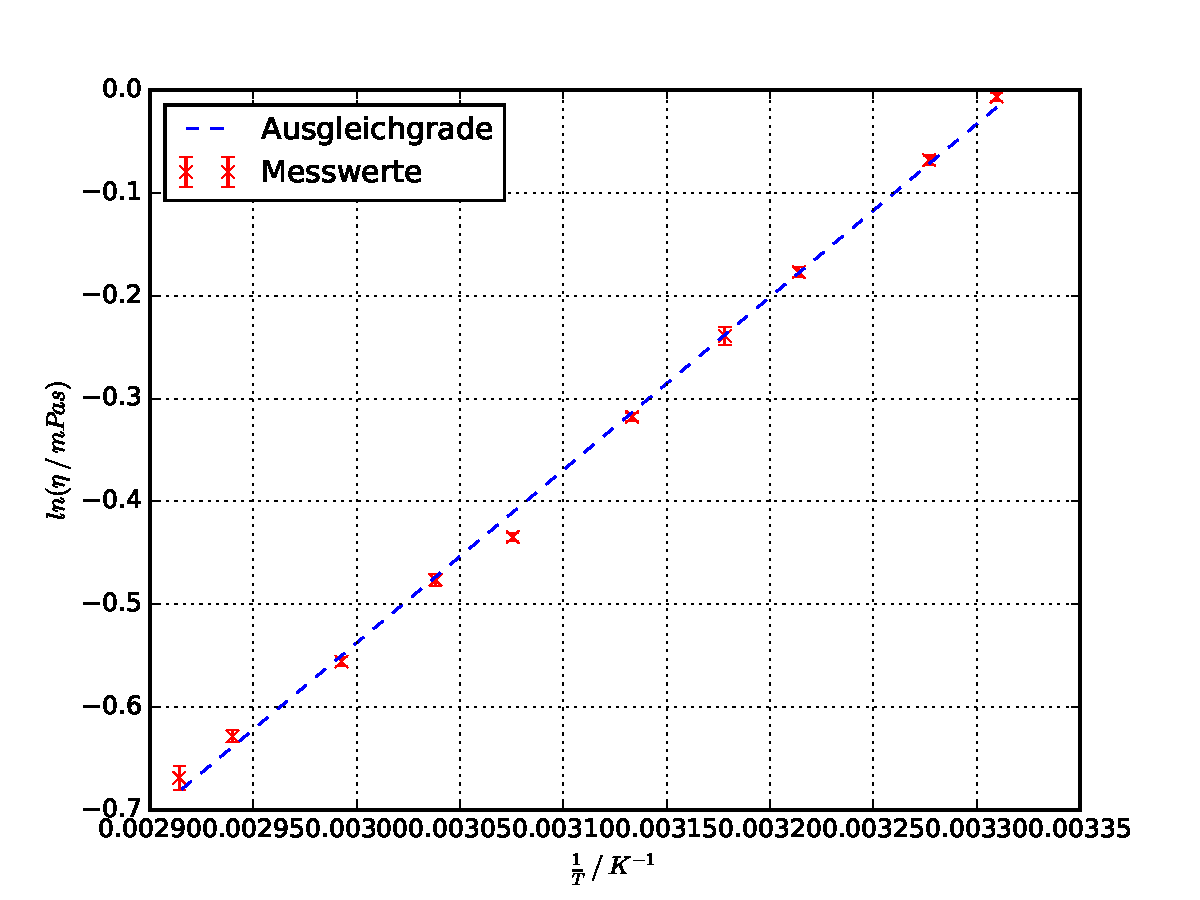
\includegraphics{plot.pdf}
%   \caption{Plot.}
%   \label{fig:plot}
% \end{figure}
\subsection{Vermessung der Fehlstellen mit dem A-Scan}
Zur erst muss die Laufzeitkorrektur $\Delta t$ bestimmt werden.
Dazu wird die Laufzeit $t$
für das Ultraschallsignal zum Boden und wieder zurück betrachtet.
Es gilt
\begin{equation*}
  H = \frac{c}{2} \left( t -\Delta t\right)
  \quad \implies \quad
  \Delta t = t - \frac{2H}{c}\;.
\end{equation*}
Dabei bezeichnet $H = \SI{8.0225}{\centi\meter}$ die Höhe des Acrylblockes
und $c$ die Schallgeschwindigkeit
in Acryl, die hier mit \SI{2730}{\meter \per \second} \cite{oly} angenommen wurde.
Daraus ergibt sich
\begin{equation*}
  \Delta t = -\SI{3.73e-7}{\second}\;.
\end{equation*}
Durch den natürlichen Zusammenhang
\begin{equation*}
  H = h_1 + h_2 + F \; ,
\end{equation*}
wobei $ h_1 $ bzw $ h_2$ den Abstand vom Rand des Blockes zur Fehlstelle
bezeichnet, folgt dann
\begin{equation}
  F = H-\frac{c}{2}\left(t_1 +t_2 - 2\Delta t \right) \; ,
  \label{eqn:F}
\end{equation}
dabei bezeichet $t_1$ bzw. $t_2$ die jeweiligen Laufzeiten des Ultraschallsignals
vom Rand des Acrylblocks und $F$ den Durchmesser der Fehlstelle. Die Messwerte
sind in den Tabellen \ref{tab:ABR} und \ref{tab:ABB} dargestellt. Die Werte
zur Vermessung der Fehlstellen in der Tabelle \ref{tab:F1}, daraus ist zu
entnehmen, dass die Fehstelle 10 nicht brechnet werden konnte da sie von
einer Seite von Fehlstelle 11 verdeckt wird und die Auflösung nicht ausreicht,
um die Fehstelle 10 dahinter aufzulösen. Zudem konnten Fehlstellen 1 und 2
nicht von einander getrennt werden, sondern wurden nur als eine Fehlstelle
interpretiert.
\begin{table}
\parbox[t]{0.48\textwidth}{
  \centering
  \caption{Messwerte der Fehlstellen von "unten"}
  \sisetup{round-mode=places, round-precision= 2}
  \begin{tabular}{S[scientific-notation= fixed, fixed-exponent = 0, round-precision = 0] S}
    \toprule
    $\text{Fehlstelle}$& $\text{Laufzeit }t$ / \si{\second} \\
    \midrule
    1.100000000000000000e+01 & 1.099999999999999971e-05\\
    9.000000000000000000e+00 & 4.539999999999999900e-05\\
    8.000000000000000000e+00 & 3.989999999999999407e-05\\
    7.000000000000000000e+00 & 3.399999999999999973e-05\\
    6.000000000000000000e+00 & 2.819999999999999767e-05\\
    5.000000000000000000e+00 & 2.210000000000000186e-05\\
    4.000000000000000000e+00 & 1.559999999999999972e-05\\
    3.000000000000000000e+00 & 9.399999999999999786e-06\\
    2.000000000000000000e+00 & 4.339999999999999782e-05\\
    1.000000000000000000e+00 & 4.339999999999999782e-05\\
    $\text{Boden}$ & 5.839999999999999651e-05\\
    \bottomrule
  \end{tabular}
  \label{tab:ABR}
  }
  \parbox[t]{0.48\textwidth}{
% \end{table}
% \begin{table}
  \centering
  \caption{Messwerte der Fehlstellen von "oben"}
  \sisetup{round-mode=places, round-precision= 2}
  \begin{tabular}{S[scientific-notation= fixed, fixed-exponent = 0, round-precision = 0] S}
    \toprule
    $\text{Fehlstelle}$& $\text{Laufzeit }t$ / \si{\second} \\
    \midrule
    1.100000000000000000e+01 & 4.009999999999999893e-05\\
    1.000000000000000000e+01 & 4.699999999999999893e-06\\
    9.000000000000000000e+00 & 1.079999999999999993e-05\\
    8.000000000000000000e+00 & 1.660000000000000031e-05\\
    7.000000000000000000e+00 & 2.239999999999999899e-05\\
    6.000000000000000000e+00 & 2.809999999999999862e-05\\
    5.000000000000000000e+00 & 3.350000000000000113e-05\\
    4.000000000000000000e+00 & 3.889999999999999686e-05\\
    3.000000000000000000e+00 & 4.449999999999999746e-05\\
    2.000000000000000000e+00 & 1.359999999999999854e-05\\
    1.000000000000000000e+00 & 1.359999999999999854e-05\\
    $\text{Boden}$ & 5.839999999999999651e-05\\
    \bottomrule
  \end{tabular}
  \label{tab:ABB}
}
\end{table}
\begin{table}
  \centering
  \caption{Werte zur Vermessung der Fehstellen}
  \sisetup{round-mode=places, round-precision= 2}
  \begin{tabular}{S[scientific-notation = fixed , fixed-exponent = 0, round-precision=0] S S S}
    \toprule
    $ \text{Fehlstellen} $& $ t_{1} $ / \si{\second}&  $ t_{2} $ / \si{\second} & $F$ /\si{\meter} \\
    \midrule
    1.100000000000000000e+01 & 4.009999999999999893e-05 & 1.099999999999999971e-05 & 9.455499999999991689e-03\\
    9.000000000000000000e+00 & 1.079999999999999993e-05 & 4.539999999999999900e-05 & 2.493999999999996220e-03\\
    8.000000000000000000e+00 & 1.660000000000000031e-05 & 3.989999999999999407e-05 & 2.084500000000003017e-03\\
    7.000000000000000000e+00 & 2.239999999999999899e-05 & 3.399999999999999973e-05 & 2.220999999999986874e-03\\
    6.000000000000000000e+00 & 2.809999999999999862e-05 & 2.819999999999999767e-05 & 2.357499999999984608e-03\\
    5.000000000000000000e+00 & 3.350000000000000113e-05 & 2.210000000000000186e-05 & 3.312999999999982625e-03\\
    4.000000000000000000e+00 & 3.889999999999999686e-05 & 1.559999999999999972e-05 & 4.814499999999999336e-03\\
    3.000000000000000000e+00 & 4.449999999999999746e-05 & 9.399999999999999786e-06 & 5.633499999999999619e-03\\
    2.000000000000000000e+00 & 1.359999999999999854e-05 & 4.339999999999999782e-05 & 1.402000000000000468e-03\\
    1.000000000000000000e+00 & 1.359999999999999854e-05 & 4.339999999999999782e-05 & 1.402000000000000468e-03\\
    \bottomrule
  \end{tabular}
  \label{tab:F1}
\end{table}
\subsection{Vermessung der Fehlstellen 1 und 2}
Das Verfahren der Vermessung der Fehlstellen 1 und 2 ist analog zu dem im
vorherigen Kapitel. Für die neue Sonde liegt die Laufzeitkorrektur bei
\begin{equation*}
  \Delta t = -\SI{1.22(05)e-6}{\second} \; .
\end{equation*}
Die 4MHz-Sonde schaft es die Fehlstellen zu trennen, somit kann mit der Formel
\eqref{eqn:F} dann der Durchmesser der Fehlstellen bestimmt werden. Die Messwerte
sind in der Tabelle \ref{tab:A2} dargestellt. Die Durchmesser der Fehlstellen
1 und 2 sind in der Tabelle \ref{tab:F2} dargestellt.

\begin{table}
  \centering
  \caption{Messwerte des Ascans mit der 4MHz-Sonde}
  \sisetup{round-mode=places, round-precision=2}
  \begin{tabular}{S[scientific-notation = fixed , fixed-exponent = 0, round-precision=0] S S}
    \toprule
    $\text{Fehlstellen}$ & $t_{1}$ /\si{\second} & $t_{2}$ /\si{\second} \\
    \midrule
    2.000000000000000000e+00 & 1.219999999999999839e-05 & 4.379999999999999399e-05\\
    1.000000000000000000e+00 & 1.340000000000000045e-05 & 4.249999999999999628e-05\\
    $\text{Boden}$ & 5.759999999999999739e-05 & 5.749999999999999496e-05\\
    \bottomrule
  \end{tabular}
  \label{tab:A2}
\end{table}
\begin{table}
  \centering
  \caption{Durchmesser der Fehlstellen 1 und 2}
  \sisetup{round-mode=places, round-precision= 0}
  \begin{tabular}{S[scientific-notation=fixed, fixed-exponent = 0, round-precision= 0] S@{$\quad \pm$\;} S}
    \toprule
    $\text{Fehlstellen}$ & \multicolumn{2}{c}{$ F \pm \Delta F$/ \si{\meter}}\\
    \midrule
    2.000000000000000000e+00 & 4.465000000000024505e-04 & 1.365000000000032908e-04\\
    1.000000000000000000e+00 & 5.830000000000001847e-04 & 1.365000000000032908e-04\\
    \bottomrule
  \end{tabular}
  \label{tab:F2}
\end{table}
\subsection{Bestimmung der Fehlstellen mit dem Bscan}
Der Durchmesser der Fehlstellen wurden wie in dem Kapitel zuvor bestimmt. Die Werte
dazu wurden in den Tabellen \ref{tab:BF1} und \ref{tab:BF2} dargestellt.
\begin{table}
  \centering
    \caption{Werte zur Vermessung der Fehstellen 3 bis 11 mit dem Bscan und der 1MHzSonde}
    \sisetup{round-mode=places, round-precision= 2}
    \begin{tabular}{S[scientific-notation = fixed , fixed-exponent = 0, round-precision=0] S S S@{$\quad\pm$} S}
      \toprule
      $ \text{Fehlstellen} $& $ t_{1} $ / \si{\second}&  $ t_{2} $ / \si{\second} & \multicolumn{2}{c}{$F \pm \Delta F$ /\si{\meter}} \\
      \midrule
      1.100000000000000000e+01 & 4.229999999999999819e-05 & 4.420000000000000372e-05 & 3.886550000000001115e-02 & 0.000000000000000000e+00\\
      1.000000000000000000e+01 & 6.999999999999999895e-06 & 8.599999999999998976e-06 & 5.791299999999999226e-02 & 0.000000000000000000e+00\\
      9.000000000000000000e+00 & 1.269999999999999868e-05 & 1.450000000000000009e-05 & 4.207899999999999141e-02 & 0.000000000000000000e+00\\
      8.000000000000000000e+00 & 1.860000000000000149e-05 & 2.039999999999999781e-05 & 2.597199999999998815e-02 & 0.000000000000000000e+00\\
      7.000000000000000000e+00 & 2.439999999999999678e-05 & 2.629999999999999892e-05 & 1.000149999999999650e-02 & 0.000000000000000000e+00\\
      6.000000000000000000e+00 & 3.019999999999999885e-05 & 3.220000000000000341e-05 & 5.969000000000002082e-03 & 0.000000000000000000e+00\\
      5.000000000000000000e+00 & 3.559999999999999797e-05 & 3.749999999999999671e-05 & 2.057449999999999557e-02 & 0.000000000000000000e+00\\
      4.000000000000000000e+00 & 4.079999999999999561e-05 & 4.289999999999999922e-05 & 3.504350000000001908e-02 & 0.000000000000000000e+00\\
      3.000000000000000000e+00 & 4.649999999999999864e-05 & 4.839999999999999739e-05 & 5.033150000000001512e-02 & 0.000000000000000000e+00\\
      \bottomrule
    \end{tabular}
    \label{tab:BF1}
\end{table}
\begin{table}
  \centering
    \caption{Werte zur Vermessung der Fehstellen 1 und 2 mit dem Bscan und der 4MHzSonde}
    \sisetup{round-mode=places, round-precision= 2}
    \begin{tabular}{S[scientific-notation = fixed , fixed-exponent = 0, round-precision=0] S S S@{$\quad \pm$} S}
      \toprule
      $ \text{Fehlstellen} $& $ t_{1} $ / \si{\second}&  $ t_{2} $ / \si{\second} & \multicolumn{2}{c}{$F \pm \Delta F$ /\si{\meter}} \\
      \midrule
      2.000000000000000000e+00 & 4.600000000000000004e-05 & 4.670000000000000350e-05 & 4.964900000000001257e-02 & 1.365000000000032908e-04\\
      1.000000000000000000e+00 & 4.459999999999999989e-05 & 4.529999999999999657e-05 & 4.582699999999999274e-02 & 1.365000000000032908e-04\\
      \bottomrule
    \end{tabular}
    \label{tab:BF2}
\end{table}
\FloatBarrier
\subsection{Untersuchung des Herzmodells}
Auch hierbei wird mit der selben Methode die Ausdehnung des Herzmodells
bestimmt. So erhält man für die maximale Ausdehnung
\begin{equation*}
  h_{max} = \SI{0.035}{\meter} \; .
\end{equation*}
Die Frequenz wurde bestimmt in dem die Zeiten zwischen den Peaks bestimmt wurde
und dann gemittelt wurden. Somit ergibt sich
\begin{equation*}
  f = \SI{2.23}{\hertz}\;.
\end{equation*}
Die Werte sind zur Veranschaulichung in der Abbildung \ref{fig:Hp} dargestellt.
Zur Bestimmung des Herzvolumens wird die ausgedehnte Membran als Paraboluid
approximiert. Das Volumen eine Paraboluiden ist gegeben durch
\begin{equation*}
  V = \frac{\pi}{2} \cdot R^2 \cdot h
\end{equation*}
daraus ergibt sich dann mit der maximalen Ausdehnung $h_{max}$ ein Volumen von
\begin{equation*}
  V = \SI{2.93e-5}{\cubic\meter}
\end{equation*}
das entspricht ca. \SI{30}{\milli\liter}.
\begin{figure}
  \centering
  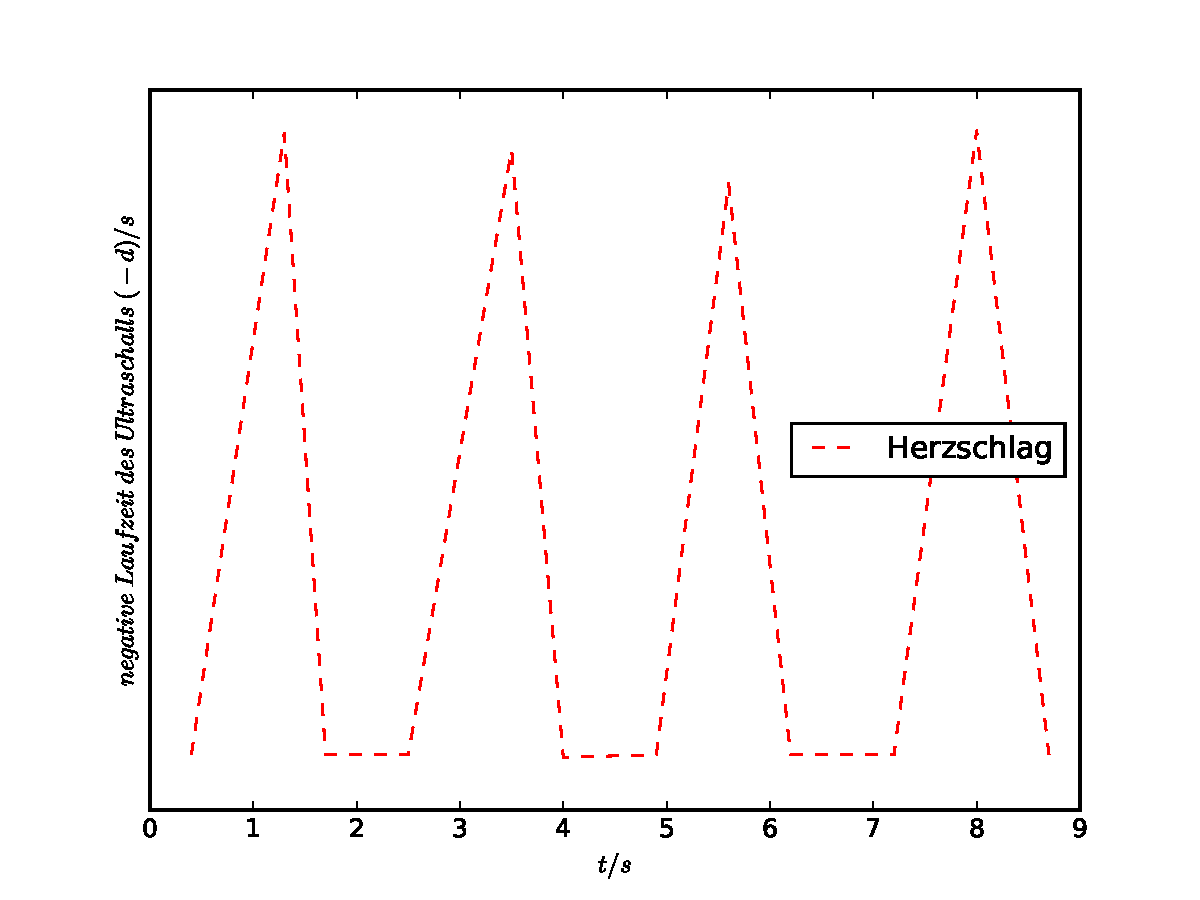
\includegraphics[height=7cm]{plots/Herzplot.pdf}
  \caption{Plot.}
  \label{fig:Hp}
\end{figure}






















%
